\chapter{Differential equations} 
The theory in this chapter is based on \cite{diffandcomplex}. In this chapter linear differential equations of the first order, separable differential equations, and their solutions will be described with corresponding examples. In this report, the Leibniz notation is used for derivatives. 
\\
\\
Before describing an RC circuit mathematically, the concept of differential equations has to be described. Differential equations are important tools to describe dynamic physical systems. An example of this could be an equation to describe an increasing population. The growth of a population is usually a function of that same population.
\begin{definition}{Differential equation}{}
A differential equation is an equation, which contains a function, and one or more of its derivatives.
\end{definition}
\noindent%Phenomena
These equations have a function as a solution, rather than a number. 
\\
A differential equation would look something like this: $\frac{dy}{dx} = y$. This equation asks: "What function is its own derivative?", which is of course $y=e^x+C$.
\\
\setlength\intextsep{0pt}
\begin{wrapfigure}{r}{7cm}[H]
	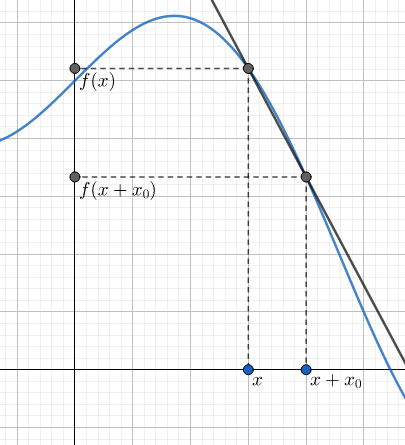
\includegraphics[scale=0.5]{fig/img/dydx.png}
	\caption{A function $f$, shown with a secant from $x$ to $x+x_0$}\label{wrap-fig:1}
\end{wrapfigure}
In this context $dy$ and $dx$ can be perceived as small changes in $y$, and small changes in $x$. The slight change in $y$, with respect to $x$, can then be described as $\dfrac{dy}{dx}$.
\\
This can be expressed formally as:
\\
\begin{align*}
	\dfrac{dy}{dx} =& y'(x) \\
	\dfrac{dy}{dx} =& \lim_{x_0\to 0} \dfrac{y(x+x_0)-y(x)}{x_0}
\end{align*}
A differential equation can either have a general solution or a particular solution. When finding the general solution, there is no initial condition to determine the constant $C$. Finding a particular solution requires an initial condition, from which the constant $C$ can be found.

\clearpage

\begin{definition}{Order of a differential equation}{}
The order of a differential equation is determined by the highest order of derivative present in the equation.
\end{definition} 

\noindent
\textbf{Examples of differential equations of different orders:}
\\
A first order differential equation:
$$y=4\frac{dy}{dx} $$
A second order differential equation:
$$\frac{d^2y}{dx^2}+\frac{dy}{dx}+y = 5\frac{dy}{dx}$$
And a third order differential equation:
$$\frac{d^3y}{dx^3} - 9\frac{d^2y}{dx^2} + 15\frac{dy}{dx} + 25y = 0$$

\section{Linear differential equations}
There are two types of differential equations, linear and non-linear. A linear differential equation is a linear polynomial that consists of a function and its derivatives.
\begin{definition}{$N$'th order linear differential equation}{}
A linear $N$'th order differential equation is an equation, which can be written in the following way:
\begin{align*}
\sum_{k=0}^{N}\left(\dfrac{d^ky}{dx^k}a_k(x)\right)+b(x)=0,
\end{align*}
where $a_k(x)$ are continuous functions on a given interval.
\end{definition}
\subsection{Solving a linear differential equation of the first order}
Solving  a differential equation is not always easy or possible. For differential equations in certain forms, a general solution can be form.

\begin{theorem}{General solution to a linear differential equation of the first order}{linethe}
A first order linear differential equation in the form of
\begin{align} \label{FODE_form}
\dfrac{dy}{dx}+h(x)y=g(x),
\end{align}
has the general solution
\begin{align} \label{FODE_solution}
y=e^{-H(x)}\left(\int e^{H(x)}g(x)\ dx+C\right),
\end{align}
where $H(x)$ is the antiderivative of $h(x)$, $h$ and $g$ are continuous in a given interval, and $C\in \mathbb{R}$.
\end{theorem}

\begin{prof}{}{}
\Cref{FODE_form} is multiplied by $e^{H(x)}$ on each side:
\begin{align*}
\left(\dfrac{dy}{dx}+h(x)y\right)e^{H(x)}=&g(x)e^{H(x)}
\\
\dfrac{dy}{dx}e^{H(x)}+h(x)ye^{H(x)}=&g(x)e^{H(x)}
\end{align*}
Considering the chain rule, and product rule, the left-hand side of the equation can be rewritten as:
\begin{align*}
\dfrac{d}{dx}\left(e^{H(x)}y\right)=g(x)e^{H(x)}
\end{align*}
This is because the left-hand side, when differentiated, becomes:
\begin{align*}
\dfrac{d}{dx}\left(e^{H(x)}y\right)=&\dfrac{d}{dx}\left(e^{H(x)}\right)y+\dfrac{dy}{dx}e^{H(x)} \\
 =& h(x)ye^{H(x)}+\dfrac{dy}{dx}e^{H(x)}
\end{align*}
Both sides are then integrated with respect to $x$:
\begin{align*}
\int\dfrac{d}{dx}\left(e^{H(x)}y\right)\ dx=&\int g(x)e^{H(x)}\ dx
\\
e^{H(x)}y=&\int g(x)e^{H(x)}\ dx+C,
\end{align*}
where $C$ is the constant of integration from the left side of the  equation. By multiplying both sides with $e^{-H(x)}$, the general solution can be found.
\begin{align}
y=e^{-H(x)}\left(\int g(x)e^{H(x)}\ dx+C\right)
\end{align}
\end{prof}

\begin{example}{Solving a linear differential equation of first order}{}
Consider the following differential equation with the given initial condition.
\begin{align}
	\dfrac{dy}{dx}-2y=e^x  \label{ODE_ex}\\ 
	y(0) =& 5 \nonumber
\end{align}
From \eqref{ODE_ex}, it is seen that it can be identified in the form of \eqref{FODE_form}, where:
%This equation can be rearranged to fit the form of \eqref{FODE_form}, and a general solution, to the differential equation, can then be found using \eqref{FODE_solution}:
\begin{align*}
	h(x) =& -2 \\
	g(x) =& e^x \\
	H(x) =& \int{-2 dx} \\
	     =& -2x + C
\end{align*}
Substituting the functions in \eqref{FODE_solution} with $H(x)$ and $g(x)$, we get: 
\begin{align*}
	y(x)=&e^{2x+C}(\int{e^{-2x-C}e^x\ dx}+C) \\
	y(x)=&e^{2x}e^{C}(e^{-C}\int{e^{-2x}e^{x}\ dx}+C) \\
	y(x)=&e^{2x}(\int{e^{-x}\ dx}+C_{1})
\end{align*}
Where $C_{1}$ is the new constant of integration, $C_1=e^{C}C$. \\
The integral of $e^{-x}$ can then be found. The following result is then reduced: